\documentclass[tikz,border=10pt]{standalone}
\usepackage{tikz,pgfplots}
\pgfplotsset{compat=1.18}

\begin{document}
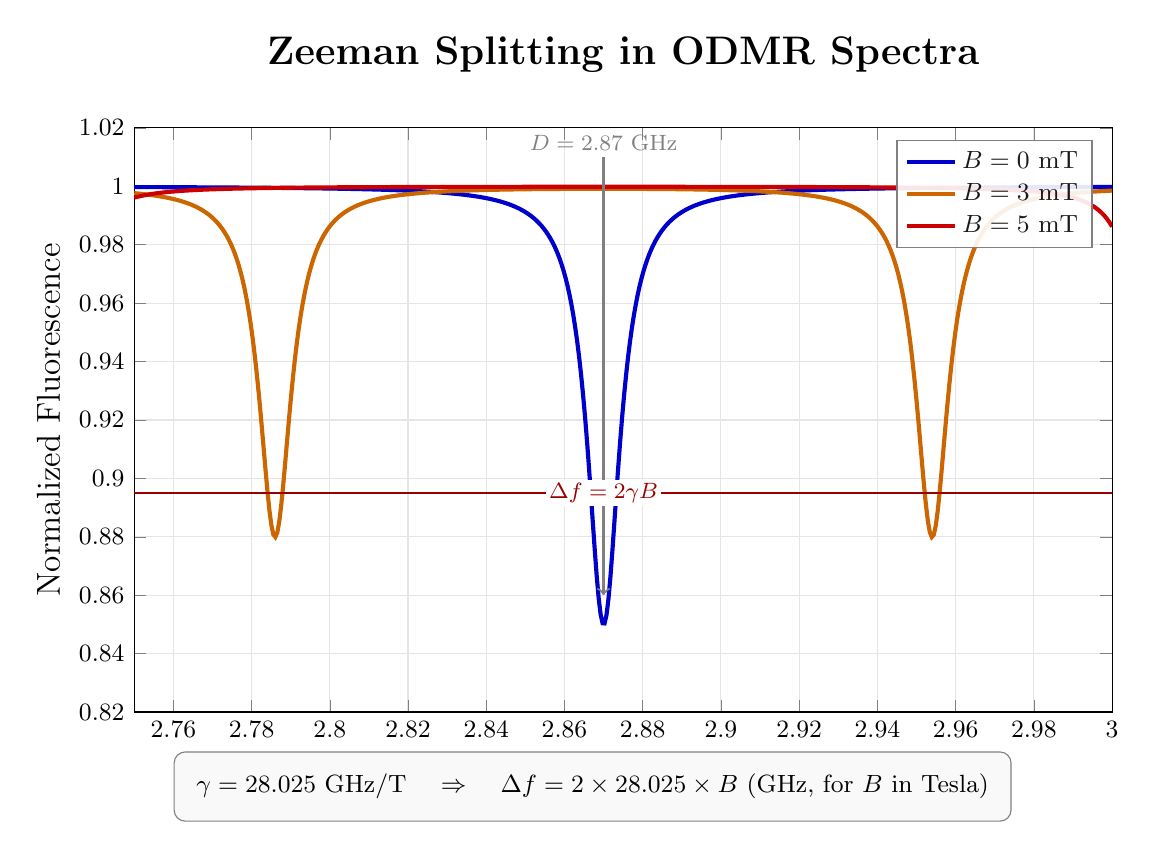
\begin{tikzpicture}

\begin{axis}[
    width=14cm,
    height=9cm,
    xlabel={\large Microwave Frequency (GHz)},
    ylabel={\large Normalized Fluorescence},
    xmin=2.75, xmax=3.0,
    ymin=0.82, ymax=1.02,
    legend style={
        at={(0.98,0.98)},
        anchor=north east,
        font=\small,
        draw=gray,
        fill=white,
        fill opacity=0.9,
    },
    grid=both,
    grid style={gray!20},
    minor grid style={gray!10},
    title={\Large\bfseries Zeeman Splitting in ODMR Spectra},
    title style={at={(0.5,1.05)}},
    tick label style={font=\small},
]

% B = 0 mT (single dip)
\addplot[
    domain=2.75:3.0,
    samples=500,
    thick,
    blue!80!black,
    line width=1.5pt,
] {1 - 0.15 * (0.005^2 / ((x - 2.87)^2 + 0.005^2))};
\addlegendentry{$B = 0$ mT}

% B = 3 mT (slight split)
\addplot[
    domain=2.75:3.0,
    samples=500,
    thick,
    orange!80!black,
    line width=1.5pt,
] {1 - 0.12 * (0.005^2 / ((x - 2.87 + 0.084)^2 + 0.005^2))
     - 0.12 * (0.005^2 / ((x - 2.87 - 0.084)^2 + 0.005^2))};
\addlegendentry{$B = 3$ mT}

% B = 5 mT (fully resolved)
\addplot[
    domain=2.75:3.0,
    samples=500,
    thick,
    red!80!black,
    line width=1.5pt,
] {1 - 0.10 * (0.004^2 / ((x - 2.87 + 0.14)^2 + 0.004^2))
     - 0.10 * (0.004^2 / ((x - 2.87 - 0.14)^2 + 0.004^2))};
\addlegendentry{$B = 5$ mT}

% Annotation: ZFS
\draw[->, thick, gray] (axis cs:2.87, 1.01) -- (axis cs:2.87, 0.86);
\node[font=\footnotesize, gray] at (axis cs:2.87, 1.015) {$D = 2.87$ GHz};

% Annotation: splitting
\draw[<->, thick, red!60!black] (axis cs:2.73, 0.895) -- (axis cs:3.01, 0.895);
\node[font=\footnotesize, red!60!black, fill=white, inner sep=1pt]
    at (axis cs:2.87, 0.895) {$\Delta f = 2\gamma B$};

\end{axis}

% Equation box
\node[draw=gray, rounded corners, fill=gray!5, inner sep=8pt,
      font=\small, anchor=north west] at (0.5, -0.5) {
    $\gamma = 28.025$ GHz/T \quad $\Rightarrow$ \quad
    $\Delta f = 2 \times 28.025 \times B$ (GHz, for $B$ in Tesla)
};

\end{tikzpicture}
\end{document}
